% Native vector cover layout with the author-approved Gaussian illustration.
% Retain chapter-figures/cover-porphine-gaussians.png when compiling.
% All positions are page-relative, independent of the chapter's text margins.
\begin{titlepage}
  \thispagestyle{empty}
  \begin{tikzpicture}[remember picture,overlay]
    \fill[hfGreenDark]
      (current page.north west) rectangle
      ([xshift=9mm]current page.south west);
    \fill[hfGreenLight]
      ([xshift=9mm,yshift=-152mm]current page.north west) rectangle
      (current page.south east);

    \node[anchor=north west,inner sep=0pt,text=hfGreenDark]
      at ([xshift=30mm,yshift=-27mm]current page.north west)
      {\sffamily\small\bfseries QUANTUM CHEMISTRY};
    \node[anchor=north east,inner sep=0pt,align=right,text=hfGreenDark]
      at ([xshift=-30mm,yshift=-24mm]current page.north east)
      {\sffamily\bfseries\fontsize{22}{24}\selectfont ESQC 2026};
    \draw[hfGreenDark,line width=0.7pt]
      ([xshift=30mm,yshift=-47mm]current page.north west) --
      ([xshift=-30mm,yshift=-47mm]current page.north east);

    \node[anchor=north west,inner sep=0pt,text=hfGreenDark]
      at ([xshift=30mm,yshift=-64mm]current page.north west)
      {\begin{minipage}{150mm}
        \raggedright
        {\fontsize{38}{43}\selectfont\bfseries
          Hartree--Fock\\Theory\par}
        \vspace{7mm}
        {\fontsize{23}{29}\selectfont
          Basis Sets and\\Molecular Integrals\par}
      \end{minipage}};

    % Approved 15 October 2026: actual normalized real s/p/d/f/g Gaussians.
    % PubChem porphine geometry; definitions and provenance are recorded in
    % drafts/cover-studies/06-porphine-exact-gaussians.md.
    % The image's transparent margins preserve the existing cover typography.
    \node[anchor=center,inner sep=0pt]
      at ([xshift=105mm,yshift=-199mm]current page.north west)
      {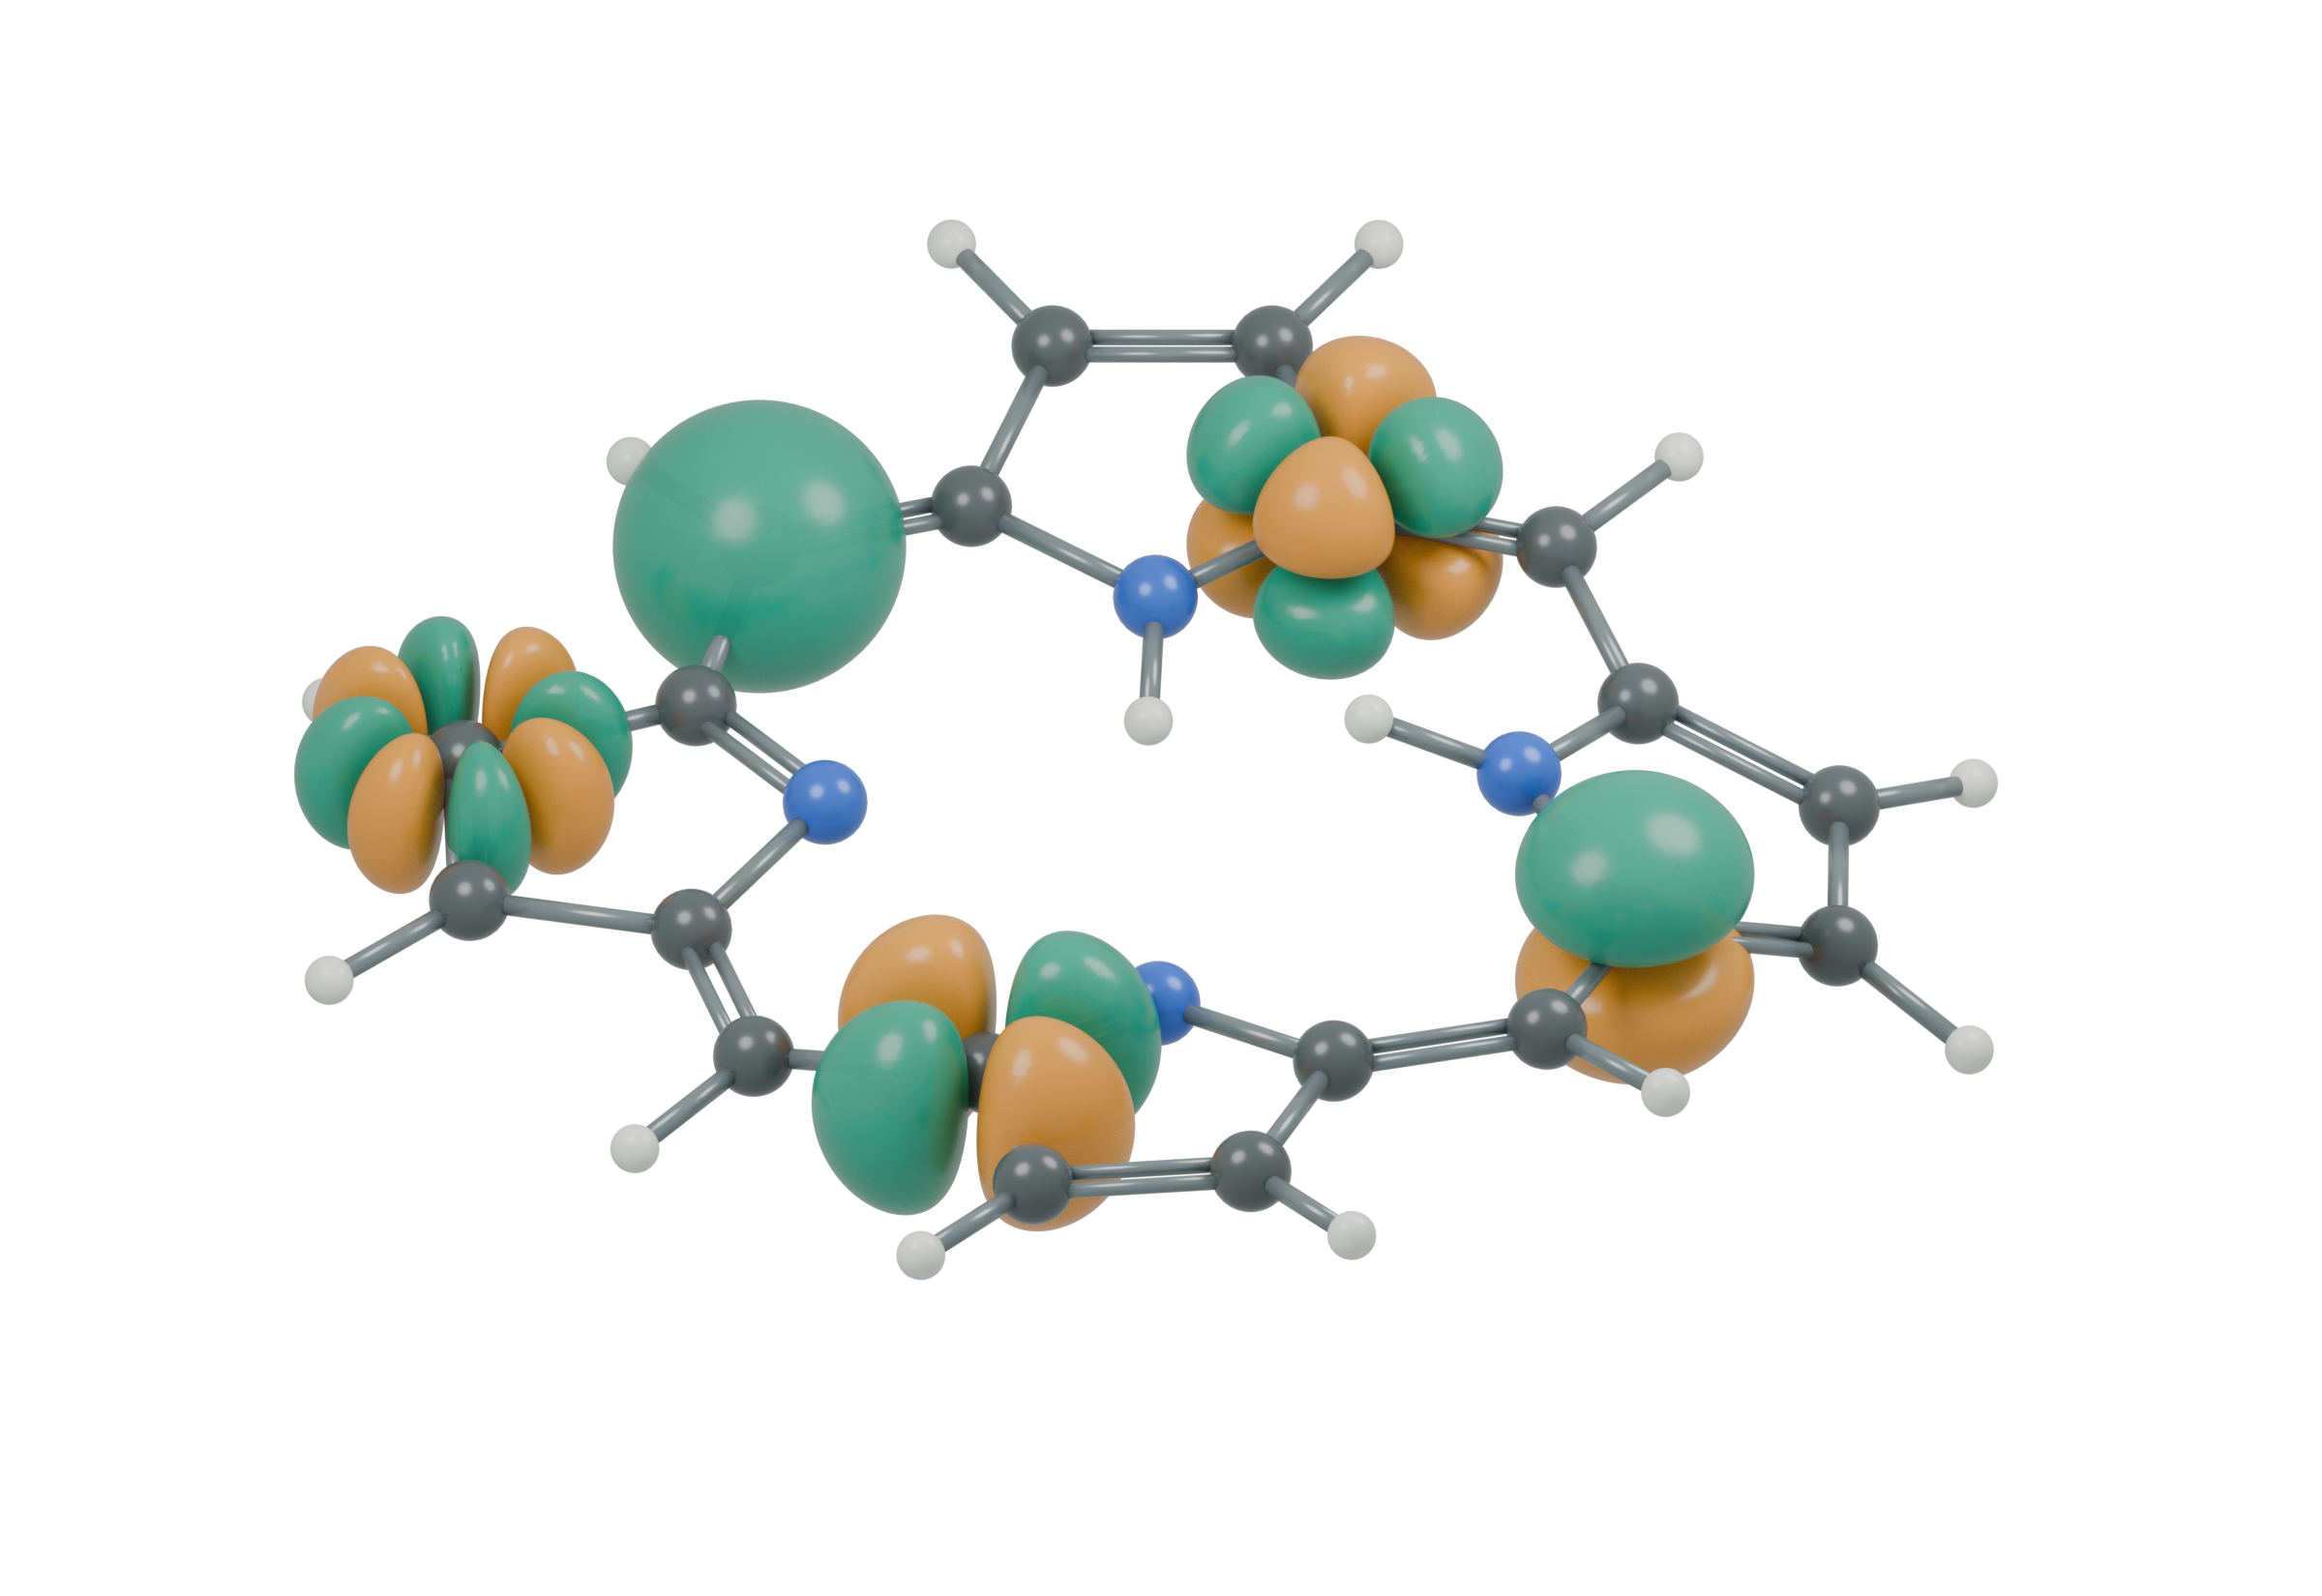
\includegraphics[width=190mm]{chapter-figures/cover-porphine-gaussians.png}};

    \node[anchor=north west,inner sep=0pt,text=hfGreenDark]
      at ([xshift=30mm,yshift=-243mm]current page.north west)
      {\begin{minipage}{150mm}
        \raggedright
        {\large\bfseries Pierre-Fran\c{c}ois (Titou) Loos\par}
        \vspace{3mm}
        {\small\color{hfInk}
          Laboratoire de Chimie et Physique Quantiques (UMR 5626)\\
          Universit\'e de Toulouse, CNRS, UPS, Toulouse, France\par}
      \end{minipage}};
    \draw[hfGreen!35,line width=0.5pt]
      ([xshift=30mm,yshift=22mm]current page.south west) --
      ([xshift=-30mm,yshift=22mm]current page.south east);
    \node[anchor=south west,inner sep=0pt,text=hfGreenDark]
      at ([xshift=30mm,yshift=14mm]current page.south west)
      {\sffamily\footnotesize European Summer School in Quantum Chemistry (ESQC)};
  \end{tikzpicture}
  \null
\end{titlepage}
